% Methodology: reproduction of OTPWR (Luo et al., Machines 2024)
% Needs in main.tex: amsmath, amssymb, array, booktabs, tikz (arrows.meta, positioning), pgfplots

The selected article proposes OTPWR, a planner that produces a short, collision-free and dynamically feasible trajectory for a differential-drive mobile robot. Our methodology follows its three stages and then reproduces them numerically (Fig.~\ref{fig:pipeline}):
(i) differential flatness reduces the planning space to the plane $(x,y)$;
(ii) an A* search with a diagonal-distance heuristic returns a shortest collision-free sequence of grid waypoints;
(iii) the waypoints are joined by piecewise polynomials whose coefficients are obtained from a convex quadratic program (QP).
Stage (iii) is the convex optimization problem at the core of the project; stages (i) and (ii) provide its inputs.

\begin{figure}[htbp]
\centering
\begin{tikzpicture}[
  node distance=0.55cm and 0.6cm,
  box/.style={draw, rounded corners=2pt, align=center, minimum height=1.1cm, text width=2.1cm, font=\small},
  core/.style={box, draw=orange!80!black, fill=orange!12, very thick},
  inp/.style={draw, dashed, rounded corners=2pt, align=center, text width=2.1cm, font=\footnotesize},
  arr/.style={-{Stealth[length=2mm]}, thick}]
\node[box] (flat) {Differential\\flatness};
\node[box, right=of flat] (astar) {Diagonal A*\\search};
\node[core, right=of astar] (qp) {Convex QP\\(minimum snap)};
\node[box, right=of qp] (cmd) {Commands\\$\theta,\ v,\ \omega$};
\node[inp, above=of flat] (robot) {Robot model\\$(x,y,\theta)$};
\node[inp, above=of astar] (map) {Grid map,\\start, goal};
\node[inp, above=of qp] (lim) {Limits\\$v_{\max},\ a_{\max}$};
\node[box, below=0.6cm of astar, text width=7.2cm, xshift=1.35cm] (val) {Validation: path length, search time, visited nodes, constraint satisfaction};
\draw[arr] (robot) -- (flat);
\draw[arr] (map) -- (astar);
\draw[arr] (lim) -- (qp);
\draw[arr] (flat) -- (astar);
\draw[arr] (astar) -- (qp);
\draw[arr] (qp) -- (cmd);
\draw[arr] (qp.south) -- (qp.south |- val.north);
\end{tikzpicture}
\caption{Methodology pipeline. Flatness reduces the robot to the plane, A* returns the waypoints $w_0,\dots,w_m$, the convex QP (highlighted) produces the smooth trajectory $x(t), y(t)$, and the flatness formulas give the commands. Only the highlighted stage is a convex optimization problem.}
\label{fig:pipeline}
\end{figure}

\subsection{Robot model and differential flatness}
The motion state of the wheeled robot in a plane has two translational components $(x,y)$ and one rotational component \( \theta \). Therefore, its kinematic equations are as follows:
\begin{equation}
\begin{bmatrix}
    \dot{x} \\
    \dot{y} \\
    \dot{\theta}
\end{bmatrix}
=
\begin{bmatrix}
    \cos\theta & 0 \\
    \sin\theta & 0 \\
    0          & 1
\end{bmatrix}
\begin{bmatrix}
    v \\
    \omega
\end{bmatrix}.
\label{eq:robot_kinematics}
\end{equation}
This system is differentially flat, because all states $(x,y,\theta)$ and control inputs $(v,\omega)$ can be expressed as a function of $x$,$y$, and their time derivatives.
In this model,the planar coordinates are chosen as flat output $\sigma = [x,\,y]^T$.
Both heading and control inputs can be recovered from the time derivatives of theses outputs for any forward motion at nonzero speed:
\begin{equation}
\theta = \arctan\frac{\dot{y}}{\dot{x}}, \qquad
v = \sqrt{\dot{x}^2+\dot{y}^2}, \qquad
\omega = \frac{\ddot{y}\dot{x}-\dot{y}\ddot{x}}{\dot{x}^2+\dot{y}^2}.
\label{eq:flatness}
\end{equation}
Due to this change of variables, the trajectory optimization can be formulated in terms of $x(t)$ and $y(t)$, having obtained $\theta$,$v$,and $\omega$ from the resulting trajectory whenever the speed is nonzero. However, when the robot starts or ends at rest,$\theta$ and $\omega$ cannot be reconstructed and therefore, these endpoints need separate treatment.

\subsection{Waypoint generation by graph search}
A two-dimensional occupancy grid is created by discretizing the environment, where the start and end goal are represented by free grid cells. Then, a path through the grid is generated using an eight connected A* search algorithm, which allows considering horizontal, vertical, and diagonal moves between neighboring cells.

The algorithm uses equation 3 to prioritize each node $n$, where the accumulated cost from the start node to node $n$ is represented by $g(n)$, and the remaining cost from node $n$ to the end goal is estimated by $h(n)$.
\begin{equation}
f(n) = g(n) + h(n), \qquad h(n) \le h^*(n),
\label{eq:astar}
\end{equation}
 The inequality (admissibility) guarantees that the returned path is the shortest one.
 Moreover, the diagonal distance heuristic for an eight connected grid, with a small tie-breaking factor $p>0$, is:
\begin{equation}
h(n) = D_s(d_x+d_y) + (D_d-2D_s)\min(d_x,d_y), \qquad h'(n) = (1+p)\,h(n),
\label{eq:heuristic}
\end{equation}
where $d_x$ and $d_y$ are the cell distances to the goal. Furthermore, this heuristic function never overestimates the true cost, as it is equal to it (Fig.~\ref{fig:grid}). However, the Manhattan distance $d_x+d_y$ may overestimate the true cost, and in result not giving the shortest path. 
This algorithm returns an ordered sequence of waypoints $\mathbf{w}_0,\ldots,\mathbf{w}_m \in \mathbb{R}^2$, where $\mathbf{w}_0$ and $\mathbf{w}_m$ are the start and end goal position. Finally, a trajectory segment is defined by a pair of consecutive waypoints. This stage is combinatorial and is not part of the convex program

\begin{figure}[htbp]
\centering
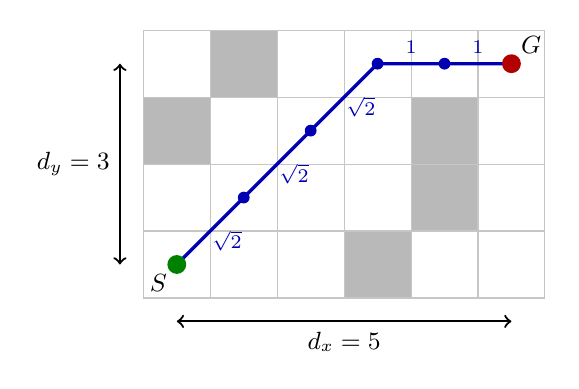
\begin{tikzpicture}[scale=0.85]
\fill[gray!55] (3,0) rectangle (4,1);
\fill[gray!55] (4,1) rectangle (5,2);
\fill[gray!55] (4,2) rectangle (5,3);
\fill[gray!55] (1,3) rectangle (2,4);
\fill[gray!55] (0,2) rectangle (1,3);
\draw[step=1, gray!45] (0,0) grid (6,4);
\draw[very thick, blue!70!black] (0.5,0.5) -- (1.5,1.5) -- (2.5,2.5) -- (3.5,3.5) -- (4.5,3.5) -- (5.5,3.5);
\foreach \p in {(1.5,1.5),(2.5,2.5),(3.5,3.5),(4.5,3.5)} \fill[blue!70!black] \p circle (2.5pt);
\fill[green!50!black] (0.5,0.5) circle (4pt) node[below left, font=\small, text=black] {$S$};
\fill[red!70!black] (5.5,3.5) circle (4pt) node[above right, font=\small, text=black] {$G$};
\node[font=\scriptsize, blue!70!black] at (1.25,0.85) {$\sqrt{2}$};
\node[font=\scriptsize, blue!70!black] at (2.25,1.85) {$\sqrt{2}$};
\node[font=\scriptsize, blue!70!black] at (3.25,2.85) {$\sqrt{2}$};
\node[font=\scriptsize, blue!70!black] at (4.0,3.75) {$1$};
\node[font=\scriptsize, blue!70!black] at (5.0,3.75) {$1$};
\draw[<->, thick] (0.5,-0.35) -- node[below, font=\small] {$d_x = 5$} (5.5,-0.35);
\draw[<->, thick] (-0.35,0.5) -- node[left, font=\small] {$d_y = 3$} (-0.35,3.5);
\end{tikzpicture}
\caption{Diagonal-distance heuristic on an 8-connected grid (grey cells are obstacles). From $S$ to $G$ ($d_x=5$, $d_y=3$) the shortest route uses three diagonal and two straight moves, of cost $3\sqrt{2}+2 \approx 6.24$, which is exactly the value of \eqref{eq:heuristic}; the Manhattan estimate $d_x+d_y=8$ is too large.}
\label{fig:grid}
\end{figure}

\subsection{Trajectory optimization problem}
The trajectory is computed separately for each axis; we present it for $x$. Segment $j=1,\dots,m$ joins $w_{j-1}$ to $w_j$ in a fixed duration $T_j$ and is a polynomial of order $n=5$ in the local time $\tau$ (Fig.~\ref{fig:segments}):
\begin{equation}
x_j(\tau) = \sum_{i=0}^{n} p_{j,i}\,\tau^{i}, \qquad \tau\in[0,T_j].
\label{eq:poly}
\end{equation}

\begin{figure}[htbp]
\centering
\begin{tikzpicture}[xscale=1.25, yscale=1.0]
\draw[-{Stealth[length=2mm]}] (0,0) -- (8.6,0) node[right, font=\small] {$t$};
\draw[-{Stealth[length=2mm]}] (0,0) -- (0,3.1) node[above, font=\small] {$x(t)$};
\foreach \t/\lab in {0/T_0, 2/T_1, 4/T_2, 6/T_3, 8/T_4} {
  \draw[dashed, gray!60] (\t,0) -- (\t,2.8);
  \node[below, font=\small] at (\t,0) {$\lab$};
}
\draw[very thick, orange!85!black] plot[smooth, tension=0.6] coordinates {(0,0.5) (2,1.9) (4,1.1) (6,2.4) (8,1.6)};
\foreach \p in {(0,0.5),(2,1.9),(4,1.1),(6,2.4),(8,1.6)} \fill[blue!70!black] \p circle (2.5pt);
\node[font=\small] at (1,2.55) {$x_1(\tau)$};
\node[font=\small] at (3,2.55) {$x_2(\tau)$};
\node[font=\small] at (5,2.85) {$x_3(\tau)$};
\node[font=\small] at (7,2.85) {$x_4(\tau)$};
\node[font=\scriptsize, blue!70!black, below right] at (2,1.9) {$w_1$};
\node[font=\scriptsize, blue!70!black, below] at (4,1.1) {$w_2$};
\end{tikzpicture}
\caption{Piecewise polynomial trajectory for one axis. Each segment $x_j(\tau)$ joins two consecutive waypoints (dots) in a duration $T_j$; at every junction the position, velocity and acceleration of neighbouring segments must agree.}
\label{fig:segments}
\end{figure}

\paragraph{Decision variables.}
The coefficients of all segments, $p = [p_1^T,\dots,p_m^T]^T \in \mathbb{R}^{m(n+1)}$. Every derivative is linear in them:
\begin{equation}
x_j^{(d)}(\tau) = r_d(\tau)^T p_j, \qquad
\big(r_d(\tau)\big)_i =
\begin{cases}
\dfrac{i!}{(i-d)!}\,\tau^{\,i-d}, & i \ge d,\\[4pt]
0, & i < d.
\end{cases}
\label{eq:derivative}
\end{equation}

\paragraph{Objective.}
The trajectory minimizes the integrated squared snap, i.e., the fourth derivative of position ($k=4$), which yields a quadratic form:
\begin{equation}
J(p) = \sum_{j=1}^{m}\int_{0}^{T_j}\big(x_j^{(4)}(\tau)\big)^2\,d\tau = \sum_{j=1}^{m} p_j^T H_j\, p_j ,
\label{eq:objective}
\end{equation}
\begin{equation}
(H_j)_{il} = \frac{i!}{(i-4)!}\,\frac{l!}{(l-4)!}\,\frac{T_j^{\,i+l-7}}{i+l-7}, \qquad i,l \ge 4,
\label{eq:H}
\end{equation}
and $(H_j)_{il}=0$ otherwise.

\paragraph{Constraints.}
The trajectory passes through the waypoints (C1), starts and ends at rest (C2), has continuous velocity and acceleration at every junction (C3), and respects the velocity and acceleration limits $v_{\max}=0.5$~m/s and $a_{\max}=0.2$~m/s$^2$ at the junctions (C4):
\begin{align}
& x_j(0) = w_{j-1}, \quad x_j(T_j) = w_j, && j=1,\dots,m, \tag{C1}\\
& \dot{x}_1(0)=\ddot{x}_1(0)=0, \quad \dot{x}_m(T_m)=\ddot{x}_m(T_m)=0, && \tag{C2}\\
& x_j^{(d)}(T_j) = x_{j+1}^{(d)}(0), \quad d=1,2, && j=1,\dots,m-1, \tag{C3}\\
& -v_{\max}\le \dot{x}_j(T_j)\le v_{\max}, \quad -a_{\max}\le \ddot{x}_j(T_j)\le a_{\max}, && j=1,\dots,m-1. \tag{C4}
\end{align}

\paragraph{Compact form.}
Stacking (C1)--(C4) gives the problem solved in the article (its Eq.~(32)):
\begin{equation}
\begin{aligned}
\min_{p}\quad & p^T H\, p\\
\text{s.t.}\quad & A p = d, \qquad B p = 0, \qquad C p \le e,
\end{aligned}
\qquad H = \operatorname{blkdiag}(H_1,\dots,H_m).
\label{eq:qp}
\end{equation}

\begin{table}[htbp]
\centering
\caption{Variables and parameters of the trajectory QP.}
\label{tab:variables}
\begin{tabular}{>{\raggedright\arraybackslash}p{2.4cm} >{\raggedright\arraybackslash}p{5.4cm} >{\raggedright\arraybackslash}p{3.4cm}}
\toprule
\textbf{Symbol} & \textbf{Meaning} & \textbf{Value / type}\\
\midrule
$p_j$ & Polynomial coefficients of segment $j$ (per axis) & Decision variable\\
$w_j$ & Waypoints from diagonal A* & Parameter\\
$T_j$ & Duration of segment $j$ & Parameter (our choice)\\
$n,\ k$ & Polynomial order, minimized derivative & $5,\ 4$ (snap)\\
$v_{\max},\ a_{\max}$ & Velocity and acceleration limits & $0.5$~m/s, $0.2$~m/s$^2$\\
$H_j$ & Snap cost matrix of segment $j$ & Positive semidefinite\\
\bottomrule
\end{tabular}
\end{table}

\subsection{Convexity analysis}
\paragraph{Objective.} For any coefficient vector, the quadratic form is an integral of a square and is therefore nonnegative:
\begin{equation}
p_j^T H_j\, p_j = \int_{0}^{T_j}\big(r_4(\tau)^T p_j\big)^2\,d\tau \;\ge\; 0 \quad \forall\, p_j
\quad\Longrightarrow\quad H_j \succeq 0 .
\label{eq:psd}
\end{equation}
Hence $H=\operatorname{blkdiag}(H_1,\dots,H_m)\succeq 0$ and $J(p)=p^THp$ is a convex quadratic function. $H$ is singular, because coefficients of degree lower than four do not appear in the snap; the objective is convex but not strictly convex, and those coefficients are fixed by the equality constraints.

\paragraph{Constraints.} (C1)--(C3) are affine equalities and (C4) are affine inequalities in $p$, so the feasible set is an intersection of hyperplanes and half-spaces, i.e., a polyhedron, which is convex.

\paragraph{Conclusion.} A convex quadratic objective minimized over a polyhedron is a convex QP. Every local minimum is therefore global and the KKT conditions are sufficient for optimality, so the solver returns the globally optimal coefficients for the given waypoints and segment times.

\subsection{Transformations, approximations and their implications}
\begin{itemize}
\item \textbf{Fixed segment times.} $T_j$ enters $H_j$ and the constraints through powers, so optimizing $p$ and $T$ jointly is non-convex. Fixing $T_j$ keeps the problem a QP; the result is optimal only for the chosen times, which the article does not report.
\item \textbf{Local time per segment.} The article writes each segment in the global time $t\in[T_{j-1},T_j]$; we use the local time $\tau = t - T_{j-1}$. Both describe the same set of trajectories, but local time avoids powers such as $65^5$ in $H_j$ and keeps the QP well conditioned.
\item \textbf{Fixed grid waypoints.} Optimality is relative to the A* path; the trajectory is forced through cell centres.
\item \textbf{Limits only at junctions.} (C4) does not prevent the velocity or acceleration from exceeding the limits inside a segment.
\item \textbf{Per-axis box limits.} $|\dot{x}|\le v_{\max}$ and $|\dot{y}|\le v_{\max}$ still allow a speed of $\sqrt{2}\,v_{\max}$.
\item \textbf{No collision constraints between waypoints.} Only the waypoints are guaranteed to be obstacle-free, and the robot is treated as a point.
\end{itemize}

\subsection{Numerical implementation}
The reproduction is implemented in MATLAB, the environment used for the article's simulations (MATLAB R2021a), with the YALMIP modeling toolbox; the QP~\eqref{eq:qp} is passed to \texttt{quadprog} (Optimization Toolbox) or to OSQP, the solver cited in the article. The workflow is:
\begin{enumerate}
\item \textbf{Map construction.} Rebuild Grid Maps~1 and~2 of the article (10~m $\times$ 10~m, 1~m cells) by reading the obstacle cells from its Figs.~7--8; start $(0.5,0.5)$~m, goal $(8.5,8.5)$~m.
\item \textbf{Path search.} Run Dijkstra ($h=0$), Euclidean A*, Manhattan A* and diagonal A*~\eqref{eq:heuristic} with $D_s=1$, $D_d=\sqrt{2}$, $p=0.001$.
\item \textbf{Segment times.} Set $T_j = \lVert w_j - w_{j-1}\rVert / \bar{v}$ with an average speed $\bar{v}=0.2$~m/s. The article does not report its times, but the path of its Fig.~9 ($6+5\sqrt{2}\approx 13.07$~m) is travelled in about $65$~s (Fig.~10), i.e., at about $0.2$~m/s.
\item \textbf{Trajectory QP.} Build $H_j$, $A$, $B$, $C$ from \eqref{eq:H} and (C1)--(C4) and solve one QP per axis.
\item \textbf{Robot commands.} Sample the polynomials and recover $\theta$, $v$ and $\omega$ from~\eqref{eq:flatness}.
\end{enumerate}

\begin{table}[htbp]
\centering
\caption{Parameters missing from the article and our choices.}
\label{tab:choices}
\begin{tabular}{>{\raggedright\arraybackslash}p{3.2cm} >{\raggedright\arraybackslash}p{3.4cm} >{\raggedright\arraybackslash}p{4.2cm}}
\toprule
\textbf{Item} & \textbf{In the article} & \textbf{Our choice}\\
\midrule
Obstacle maps & Figures only & Read from Figs.~7--8\\
Move costs $D_s$, $D_d$ & Not stated & $1$ and $\sqrt{2}$ (match $12.4853 = 4+6\sqrt{2}$)\\
Tie-break factor $p$ & \emph{small, close to zero} & $0.001$\\
Segment times $T_j$ & Not given & Segment length $/\,0.2$~m/s (inferred from Figs.~9--10)\\
Solver & OSQP & \texttt{quadprog} or OSQP via YALMIP\\
\bottomrule
\end{tabular}
\end{table}

\subsection{Validation and evaluation}
The reproduction is validated against the article's reported results:
\begin{itemize}
\item \textbf{Path search} (Tables~1--2 of the article): path length, search time and number of visited nodes for the four algorithms (Fig.~\ref{fig:benchmarks}). Path lengths should match exactly ($12.4853$~m and $13.8995$~m); search times depend on the computer, so rankings and ratios are compared.
\item \textbf{Trajectory} (Figs.~9--12 of the article, on a third map that we rebuild from Fig.~9): smoothness of the trajectory, total duration of about $65$~s, per-axis velocity and acceleration within $\pm0.5$~m/s and $\pm0.2$~m/s$^2$, and the commands $v$ and $\omega$.
\item \textbf{Feasibility checks:} solver status, satisfaction of (C1)--(C4), and the maximum velocity and acceleration inside each segment.
\end{itemize}
Any significant discrepancy with the published numbers will be identified and explained.

\begin{figure}[htbp]
\centering
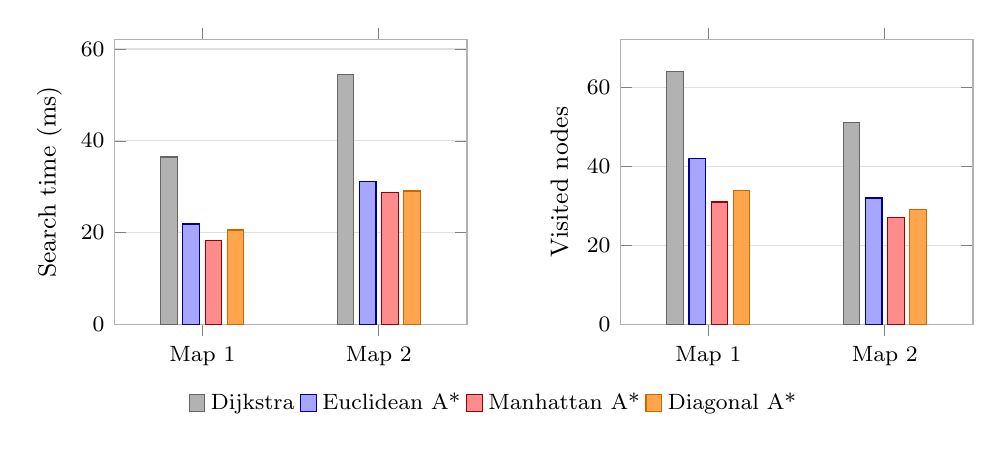
\begin{tikzpicture}
\pgfplotsset{
  bench/.style={ybar, width=0.5\textwidth, height=5.2cm, bar width=6pt,
    symbolic x coords={Map 1, Map 2}, xtick=data, ymin=0, enlarge x limits=0.5,
    tick label style={font=\footnotesize}, label style={font=\small},
    ymajorgrids, grid style={gray!25}, axis line style={gray!60}}
}
\begin{axis}[bench, ylabel={Search time (ms)}, ymax=62,
  legend style={at={(1.08,-0.2)}, anchor=north, legend columns=4, font=\footnotesize, draw=none},
  legend image code/.code={\draw[#1] (0cm,-0.1cm) rectangle (0.2cm,0.12cm);}]
\addplot[fill=gray!60, draw=gray!80!black] coordinates {(Map 1,36.5) (Map 2,54.5)};
\addplot[fill=blue!35, draw=blue!60!black] coordinates {(Map 1,21.9) (Map 2,31.2)};
\addplot[fill=red!45, draw=red!60!black] coordinates {(Map 1,18.4) (Map 2,28.7)};
\addplot[fill=orange!70, draw=orange!80!black] coordinates {(Map 1,20.6) (Map 2,29.1)};
\legend{Dijkstra, Euclidean A*, Manhattan A*, Diagonal A*}
\end{axis}
\begin{axis}[bench, xshift=0.53\textwidth, ylabel={Visited nodes}, ymax=72]
\addplot[fill=gray!60, draw=gray!80!black] coordinates {(Map 1,64) (Map 2,51)};
\addplot[fill=blue!35, draw=blue!60!black] coordinates {(Map 1,42) (Map 2,32)};
\addplot[fill=red!45, draw=red!60!black] coordinates {(Map 1,31) (Map 2,27)};
\addplot[fill=orange!70, draw=orange!80!black] coordinates {(Map 1,34) (Map 2,29)};
\end{axis}
\end{tikzpicture}
\caption{Published path-search benchmarks of the article (its Tables~1--2) that the reproduction will be compared with. Manhattan A* is fastest but returns a longer path on Map~2 ($14.4853$~m instead of $13.8995$~m); diagonal A* always finds the shortest path and, on Map~2, is $46.6\%$ faster than Dijkstra with $43.1\%$ fewer visited nodes.}
\label{fig:benchmarks}
\end{figure}

\subsection{Planned extensions}
Each extension keeps the problem convex:
\begin{itemize}
\item \textbf{E1 -- True speed limit (SOCP).} Replace the per-axis boxes by a norm bound that couples $x$ and $y$ at sample times $\tau_s$, which is a second-order cone constraint:
\begin{equation}
\big\lVert [\dot{x}_j(\tau_s),\ \dot{y}_j(\tau_s)] \big\rVert_2 \le v_{\max}.
\label{eq:soc}
\end{equation}
\item \textbf{E2 -- Limits inside segments.} Impose (C4) at several sample times in each segment (still a QP).
\item \textbf{E3 -- Safe corridors.} Keep sampled positions inside obstacle-free rectangles around each segment (linear inequalities, still a QP).
\item \textbf{E4 -- Sensitivity analysis.} Compare minimum jerk ($k=3$) with minimum snap ($k=4$), and vary the segment times and the limits.
\end{itemize}
